\documentclass{article}
\usepackage[utf8]{inputenc}
\usepackage{import}
\usepackage[subpreambles=true]{standalone}
\usepackage{graphicx}
\usepackage{amsmath}
\usepackage{amsfonts}
\usepackage{amssymb}
\usepackage{mathrsfs}
\usepackage{enumerate}
\usepackage{fancyhdr}
\usepackage[colorlinks=true,linkcolor=black,anchorcolor=black,citecolor=black,filecolor=black,menucolor=black,runcolor=black,urlcolor=blue]{hyperref}
\usepackage[margin=1.75in]{geometry}
\usepackage{algorithm, algpseudocode}
\usepackage{tikz-qtree}
\usepackage{ulem}

\tikzstyle{arr}=[fill=white, draw=black, shape=rectangle, scale=.85]
\tikzstyle{cir}=[fill=white, draw=black, shape=circle, scale=.75]

\begin{document}
%%%%%%%%%%%%%%%%%%%%%%%%%%%%
%%     Chapter Content    %%
%%%%%%%%%%%%%%%%%%%%%%%%%%%%
\section{Quicksort}
\rule{\textwidth}{1pt}\\
\subsection{Pseudocode}
\begin{algorithm}
\caption{Quicksort}
\begin{algorithmic}[1]
\Procedure{quicksort}{$A, p, r$}
	\If{$p<r$}
		\State $q\leftarrow$ \Call{partition}{$A, p, r$}
		\State \Call{quicksort}{$A, p, q-1$}
		\State \Call{quicksort}{$A, q+1, r$}
	\EndIf
\EndProcedure
\Statex
\Function{partition}{$A, p, r$}
	\State $X\leftarrow A[r]$
	\State $i\leftarrow p-1$
	\For {$j=p$ \textbf{ to } $r-1$}
		\If{$A[j] \leq X$}
			\State $i\leftarrow i+1$
			\State $A[i]\leftrightarrow A[j]$
		\EndIf
	\EndFor
	\State $A[i+1]\leftrightarrow A[r]$
	\State \Return $(i+1)$
\EndFunction
\end{algorithmic}
\end{algorithm}

\subsection{Analysis}
The worst case is when the pivot is either in the \textit{first} or \textit{last} index, 
best case is when the pivot is the \textit{median} index, and the "average" case is when the pivot
is between the first/last and median index (here $q$ will represent the \textit{true} average).
\begin{center}
	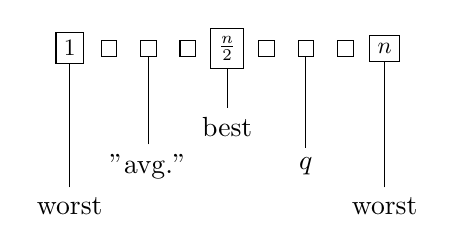
\begin{tikzpicture}
		\node [style=arr] (1) at (0, 0) {1};
		\node [style=arr] (2) at (0.5, 0) {};
		\node [style=arr] (3) at (1, 0) {}; 
		\node [style=arr] (4) at (1.5, 0) {};
		\node [style=arr] (5) at (2, 0) {$\frac{n}{2}$};
		\node [style=arr] (6) at (2.5, 0) {};
		\node [style=arr] (7) at (3, 0) {};
		\node [style=arr] (8) at (3.5, 0) {};
		\node [style=arr] (9) at (4, 0) {$n$};

		\node (10) at (0, -2) {worst};
		\node (11) at (2, -1) {best};
		\node (12) at (1, -1.5) {"avg."};
		\node (20) at (4, -2) {worst};
		\node (22) at (3, -1.5) {$q$};

		\draw (10) to (1);
		\draw (20) to (9);
		\draw (11) to (5);
		\draw (12) to (3);
		\draw (22) to (7);
	\end{tikzpicture}
\end{center}

\subsubsection*{Worst Case}
	As a recurrence,
	\begin{align*}
		T(n) &= T(n-1) + n-1, \hspace{3mm} T(0)=T(1)=0 \\
		&= \sum_{i=1}^{n-1} i = \frac{(n-1)n}{2}
	\end{align*}

\subsubsection*{Best Case}
	As a recurrence,
	\begin{align*}
		T(n) &= 2T\left(\frac{n}{2}\right) + n-1, \hspace{3mm} T(0)=T(1)=0 \\
		&= n\lg n - n + 1
	\end{align*}
	Note: This is the same recurrence as Mergesort!

\subsubsection*{Average Case}
	As a recurrence,
	\begin{align*}
		T(n) &= T\left(\frac{n}{4}\right) + T\left(\frac{3n}{4}\right) + n-1, \hspace{3mm} T(0)=T(1)=0 %\\
		%&\lesssim 1.23n\lg n
	\end{align*}
	Solve with Strong Constructive Induction. \\
	Guess: $T(n) \leq an\lg n$ for $n\geq 1$ and some constant $a$. \\
	Base case $n=1$: $an\lg n = a1\lg 1 = a\cdot 1\cdot 0 = 0$, $T(1) = 0$ and $0\leq 0$. \\
	Inductive Hypothesis: Assume true for $< n$, $T(k) \leq ak\lg k$ for $1\leq k\leq n$. \\
	Inductive Step:
		\begin{align*}
			T(n) &= T\left(\frac{n}{4}\right) + T\left(\frac{3n}{4}\right) + n-1 \\
			&\leq a\frac{n}{4}\lg\left(\frac{n}{4}\right) + a\frac{3n}{4}\lg\left(\frac{3n}{4}\right) + n-1 \hspace{5mm}\text{by IH} \\
			&\leq a\frac{n}{4}\left(\lg n - \lg 4\right) + a\frac{3n}{4}\left(\lg 3 + \lg n - \lg 4\right) + n-1 \\
			&\leq \frac{an}{4}\left(\lg n - 2\right) + \frac{3an}{4}\left(\lg 3 +\lg n - 2\right) + n-1 \\
			&\leq \frac{an\lg n}{4} - \frac{2an}{4} + \frac{3an\lg3}{4} + \frac{3an\lg n}{4} - \frac{2\cdot 3an}{4} + n-1 \\
			&\leq an\lg n + \left(-\frac{a}{2} + \frac{3a\lg 3}{4}- \frac{3}{2}a + 1\right)n -1 \\
			&\leq an\lg n + \left(\left(\frac{3\lg3}{4}-2\right)a + 1\right)n -1
		\end{align*}
	It follows that we need 
	$$\left(\frac{3\lg 3}{4}-2\right)a + 1\leq 0 \implies a \geq \frac{1}{2 - \frac{3\lg 3}{4}}$$
	$$a \gtrsim 1.23$$
	Thus, 
	$$T(n) \lesssim 1.23 n\lg n$$

\subsubsection*{Exact Average Case}
	As a recurrence,
	\begin{align*}
		T(n) &= \left[\sum_{q=1}^{n} \frac{1}{n} \Big(T(q-1) + T(n-q)\Big)\right] + n-1, \hspace{3mm} T(0)=T(1)=0 \\
		&= \frac{1}{n} \sum_{q=1}^{n} \Big(T(q-1) + T(n-q)\Big) + n-1 \\
		&= \frac{1}{n} \sum_{q=1}^{n} T(q-1) + \frac{1}{n}\sum_{q=1}^{n} T(n-q) + n-1 \\
		&= \frac{1}{n} \sum_{q=0}^{n-1} T(q) + \frac{1}{n}\sum_{q=0}^{n-1} T(q) + n-1^{*} \\
		&= \frac{2}{n} \sum_{q=0}^{n-1} T(q) + n-1
	\end{align*}
	$^{*}$Note that: 
	\begin{align*}
		\sum_{q=1}^{n} T(q-1) &= T(0) + T(1) + T(2) + \cdots + T(n-1) \\
		\sum_{q=1}^{n} T(n-q) &= T(n-1) + T(n-2) + T(n-3) + \cdots + T(0)
	\end{align*}
	Solve with Strong Constructive Induction. \\
	Guess: $T(n) \leq an\lg n$ for $n\geq 1$ and some constant $a$. \\
	Base case $n=1$: $an\lg n = a1\lg 1 = a\cdot 1\cdot 0 = 0$, $T(1) = 0$ and $0\leq 0$. \\
	Inductive Hypothesis: Assume true for $< n$, $T(k) \leq ak\lg k$ for $1\leq k\leq n$. \\
	Inductive Step:
	\begin{align*}
		T(n) &= n-1 + \frac{2}{n} \sum_{q=0}^{n-1} T(q) \\
		&= n-1 + \frac{2}{n} \sum_{q=1}^{n-1} T(q) \\
		&\leq n-1 + \frac{2}{n} \sum_{q=1}^{n-1} aq\lg q \hspace{5mm}\text{by IH} \\
		&\leq n-1 + \frac{2a}{n}\int_{1}^{n} x\lg x dx \hspace{5mm}\text{by integral bound} \\
		&= n-1 + \frac{2a}{n} \left[\frac{x^2\lg x}{2} - \frac{x^2\lg e}{4}\right] \Big|_1^n \\
		&= n-1 + an\lg n - \frac{an\lg e}{2} + \frac{a\lg e}{2n} \\
		&= an\lg n + \left[1- \frac{a\lg e}{2}\right]n - 1 + \frac{a\lg e}{2n}
	\end{align*}
	It follows that we need
	$$1 - \frac{a\lg e}{2} \leq 0 \implies a\geq \frac{2}{\lg e}$$
	So set $a = \frac{2}{\lg e} \approx 1.39$, we then need
	$$\frac{a\lg e}{2n}-1 \leq 0 \iff \frac{2\lg e}{(\lg e) 2n} -1 \leq 0 \iff \frac{1}{n}-1 \leq 0$$
	Thus, 
	$$T(n) \lesssim 1.39n\lg n$$
	We can realize a more natural formula,
	$$T(n) \leq an\lg n = \frac{2n\lg n}{\lg e} = 2n\ln n$$
	\textbf{Theorem}\\
	\textit{The expected number of comparisons for Quicksort is $\approx 2n\ln n$.}

\subsubsection*{Blum's Exact Average Case}
	Let $P(i,j)$ be the probability that the $i$th smallest and $j$th smallest elements are compared. \\\\
	\textbf{Theorem}\\
	\textit{The average number of comparisons for quicksort is}
	$$\sum_{1\leq i<j \leq n} P(i,j)$$
	Only matters the first time an element from $A[i],\cdots, A[j]$ is picked as pivot.
	The probability that the $i$th and $j$th smallest elements are compared during the execution of
	quicksort is:
	$$\frac{2}{j-i+1}$$
	Then,
	\begin{align*}
		\sum_{1\leq i<j \leq n} P(i,j) &= \sum_{i=1}^n \sum_{j=i+1}^n P(i,j) = \sum_{i=1}^n \sum_{j=i+1}^n \frac{2}{j-i+1} \\
		&= 2\sum_{i=1}^n \sum_{j=i+1}^n\frac{1}{j-i+1} \\
		&= 2\sum_{i=1}^n \left(\frac{1}{2} + \frac{1}{3} + \cdots + \frac{1}{n-i+1}\right) \\
		&= 2\sum_{i=1}^n \left(H_{n-i+1} -1\right) = 2\sum_{i=1}^n H_{n-i+1} - 2\sum_{i=1}^n 1 \\
		&= 2(H_n + H_{n-1}+ \cdots + H_1) - 2\sum_{i=1}^n 1 \\
		&= 2\sum_{i=1}^n H_i -2n \\
		&= 2((n+1)H_n -n) -2n \\
		&= 2(n+1)H_n -4n \approx 2n\ln n
	\end{align*}

\subsection{Comments}
\subsubsection*{Quicksort Code}
Recall the Quicksort procedure,
\begin{algorithmic}
	\Procedure{quicksort}{$A, p, r$}
		\If{$p<r$}
			\State $q\leftarrow$ \Call{partition}{$A, p, r$}
			\State \Call{quicksort}{$A, p, q-1$}
			\State \Call{quicksort}{$A, q+1, r$}
		\EndIf
	\EndProcedure
\end{algorithmic}
When executing quicksort$(A, p, q-1)$ we must stack up quicksort$(A,q+1, r)$ to be executed later.
We need to store the pair of index values $(q+1, r)$.
\subsubsection*{Stack in Action}
The left table represents the pivot being the largest element, and the right
table represents the pivot being the smallest element.
\begin{table}[!htb]
\centering
\begin{tabular}{lllll}
 \textbf{Pivot} & \textbf{Stack} &  & \textbf{Pivot} & \textbf{Stack} \\
 $A[n]$ & $(n+1,n)$ &  & $A[1]$ & \sout{$(2,n)$} \\
 $A[n-1]$& $(n,n-1)$ &  & $A[2]$ & \sout{$(3, n)$} \\
 $A[n-2]$& $(n-1,n-2)$ &  & $A[3]$ & \sout{$(4, n)$} \\
 $\vdots$ & $\vdots$ &  & $\vdots$ & $\vdots$ \\
 $A[3]$& $(4,3)$ &  & $A[n-2]$ & \sout{$(n-1, n)$} \\
 $A[2]$& $(3,2)$ &  & $A[n-1]$ & \sout{$(n, n)$} \\
 $A[1]$ &  &  & $A[n]$ & 
\end{tabular}
\end{table} \\
When the pivot is the smallest element the stack remains very small
but if the pivot is the largest element we stack $n-1$ problems to do later.
\subsubsection*{In Place}
On average, height of the stack for Quicksort is $\Theta (\log n)$.
Height of stack for Mergesort is $\lg n + O(1)$. \\\\
\textbf{Definition:}
An algorithm is \textit{in place} if it uses $O(1)$ extra variables and
(on average) $O(\log n)$ extra index variables. \\\\
A more technical definition is;
An algorithm is \textit{in place} if it uses at most $O(1)$ extra variables
and (on average) $O\left((\log n)^2\right)$ extra bits.
\subsubsection*{Stack}

We can modify the Quicksort procedure so that stack has height at most $\lg n$.
\begin{algorithmic}
	\Procedure{quicksort}{$A, p, r$}
		\If{$p<r$}
			\State $q\leftarrow$ \Call{partition}{$A, p, r$}
			\If{$q\leq (p+r)/2$}
				\State \Call{quicksort}{$A, p, q-1$}
				\State \Call{quicksort}{$A, q+1, r$}
			\Else
				\State \Call{quicksort}{$A, q+1, r$}
				\State \Call{quicksort}{$A, p, q-1$}
			\EndIf
		\EndIf
	\EndProcedure
\end{algorithmic}
\subsubsection*{Is Quicksort In Place?}
Quicksort is in place, but it does not use a constant amount of extra space.
Quicksort uses slightly more than a constant amount of extra space.
\subsubsection*{Choice of Pivots}
It is risky to pivot on the last element because the last element could be
the largest element. Some better ways could be;
\begin{itemize}
	\item Pivot on middle element.
	\item Pivot on median of first, middle, and last elements.
	\item Pivot on random element.
	\item Pivot on median of three random elements.
	\item Pivot on median of five random elements. (Law of diminishing returns.)
	\item Randomly permute array before starting. (Equivalent to pivoting on random element.)
\end{itemize}
\subsubsection*{Partitioning}
There are a variety of partition routines. The current edition of the textbook has a version
that uses $n-1$ comparisons, but the previous edition of the textbook has a version which uses
$n$ comparisons.

\end{document}